%! suppress = TooLargeSection
\documentclass[conference]{IEEEtran}
\usepackage{cite}
%\usepackage{amsmath,amssymb,amsfonts}
\usepackage{algorithmicx}
\usepackage{graphicx}
\usepackage{textcomp}
\usepackage{xcolor}

\usepackage{subfig}
\usepackage[hidelinks]{hyperref}
\graphicspath{ {images/} }
\usepackage{pgfplots}
\usepackage{tikz}
\pgfplotsset{compat=1.17}

\newcommand\BibTeX{{\textrm{B} \kern-.05em{\textsc{i} \kern-.025em b}\kern-.08em
T\kern-.1667em\lower.7ex\hbox{E}\ker,n-.125emX}}

\begin{document}

    \title{E\textsubscript{in-style}: Clothing Item Generation using GANs}

    \author{\IEEEauthorblockN{Charlie Brayton (014559415)}
    \IEEEauthorblockA{\textit{Department of Software Engineering} \\
    \textit{San José State University}\\
    San José, California \\
    charles.brayton@sjsu.edu}
    \and
    \IEEEauthorblockN{Mohit Patel (014501461)}
    \IEEEauthorblockA{\textit{Department of Software Engineering} \\
    \textit{San José State University}\\
    San José, California \\
    mohit.patel@sjsu.edu}
    \and
    \IEEEauthorblockN{Andrew Selvia (014547273)}
    \IEEEauthorblockA{\textit{Department of Software Engineering} \\
    \textit{San José State University}\\
    San José, California \\
    andrew.selvia@sjsu.edu}
    \and
    \IEEEauthorblockN{Dylan Zhang (013073437)}
    \IEEEauthorblockA{\textit{Department of Software Engineering} \\
    \textit{San José State University}\\
    San José, California \\
    dylan.zhang@sjsu.edu}
    }

    \maketitle

    \begin{abstract}

        The primary objective of this research is to classify and generate images of clothing items.\ It is a compilation of three distinct efforts: (1) to classify fashion-mnist~\cite{xiao2017/online} images and, inversely, add adversarial noise to test the classifier; (2) to generate novel images which emulate the true fashion-mnist images;\ (3) to infuse the grayscale images with life-like colors.\ Together, these endeavours pushed the team to explore topics at the forefront of modern machine learning, especially generative adversarial networks (GANs).

    \end{abstract}

    \begin{IEEEkeywords}
        machine learning, computer vision, neural networks, generative adversarial networks
    \end{IEEEkeywords}

    \section{Introduction}\label{sec:introduction}

    The diverse branches of this project were made possible by the careful selection of a dataset.\ The fashion-mnist dataset was chosen specifically for its prevalence as a benchmark in recent research into neural networks.\ Its size, labels, and compatibility (with the long-established MNIST dataset) make it an ideal choice for evaluating deep neural networks (NNs) and GANs. Rather than attempt to introduce a truly groundbreaking NN architecture given the authors' limited experience, this project aims for breadth.

    Each subproject explores a unique research area with industrial applications which may answer the associated questions:

    \begin{enumerate}
        \item Classification: Can we quickly identify an item of clothing to automate sorting and retrieval?\ Supposing such an automated system existed, how susceptible might it be to failure?
        \item Generation: Can the product development lifecycle for clothing be accelerated by avoiding physical prototyping?
        \item Colorization: Can grayscale clothing imagery be augmented with colors to enable A/B testing of styles to increase customer satisfaction?
    \end{enumerate}

    To aid comprehension, each subproject is explored independently.

    \section{Data}\label{sec:data}

    The fashion-mnist dataset~\cite{xiao2017/online} is composed of 60,000 training images and 10,000 testing images.\ In keeping with the legacy of the traditional MNIST, fashion-mnist images are 28x28 grayscale pixels.\ Each image is labeled as one of the ten classes pictured in \autoref{fig:fashion-mnist} and enumerated below:

    \begin{enumerate}
        \setcounter{enumi}{-1}
        \item T-shirt/top
        \item Trouser
        \item Pullover
        \item Dress
        \item Coat
        \item Sandal
        \item Shirt
        \item Sneaker
        \item Bag
        \item Ankle Boot
    \end{enumerate}

    \begin{figure}
        \caption{fashion-mnist Samples}
        \label{fig:fashion-mnist}
        \begin{center}
            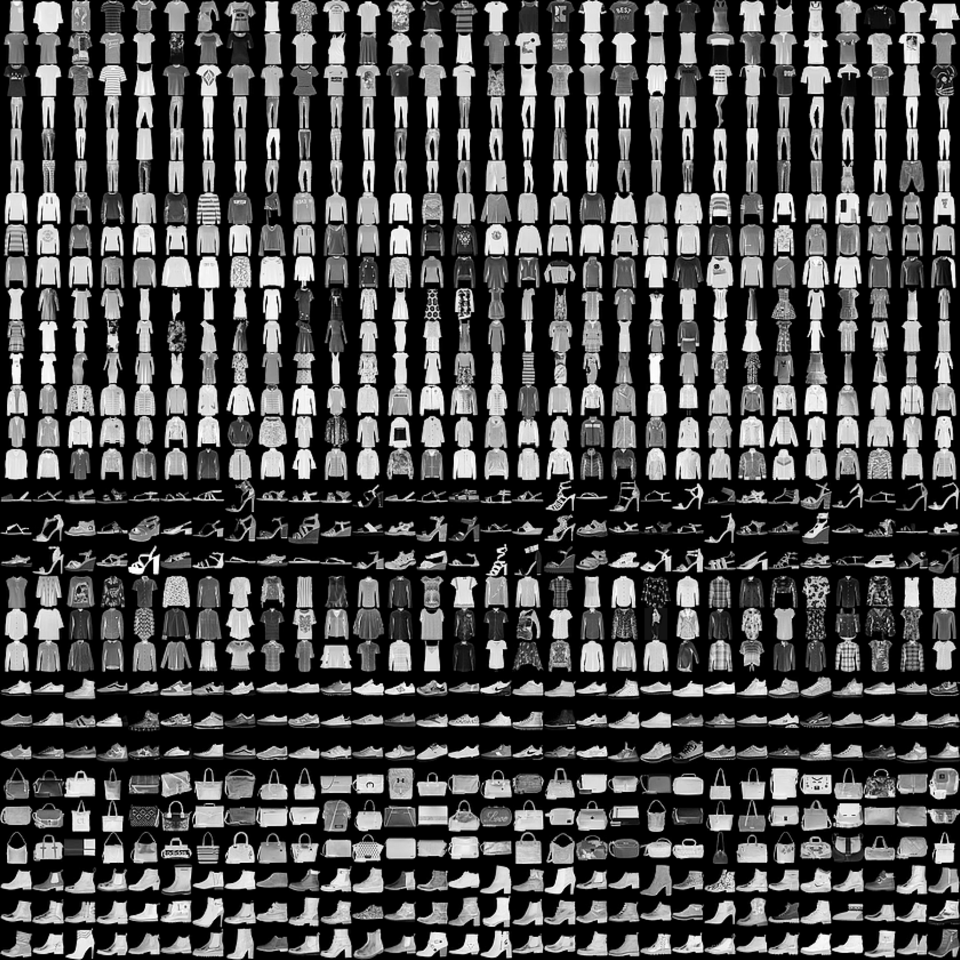
\includegraphics[width=0.45\textwidth]{data.png}
        \end{center}
    \end{figure}

    \section{Implementation}\label{sec:implementation}

    \subsection{Classification}\label{subsec:implementation-classification}

    \begin{figure}
        \caption{Classified fashion-mnist Testing Images}
        \label{fig:classification}
        \begin{center}
            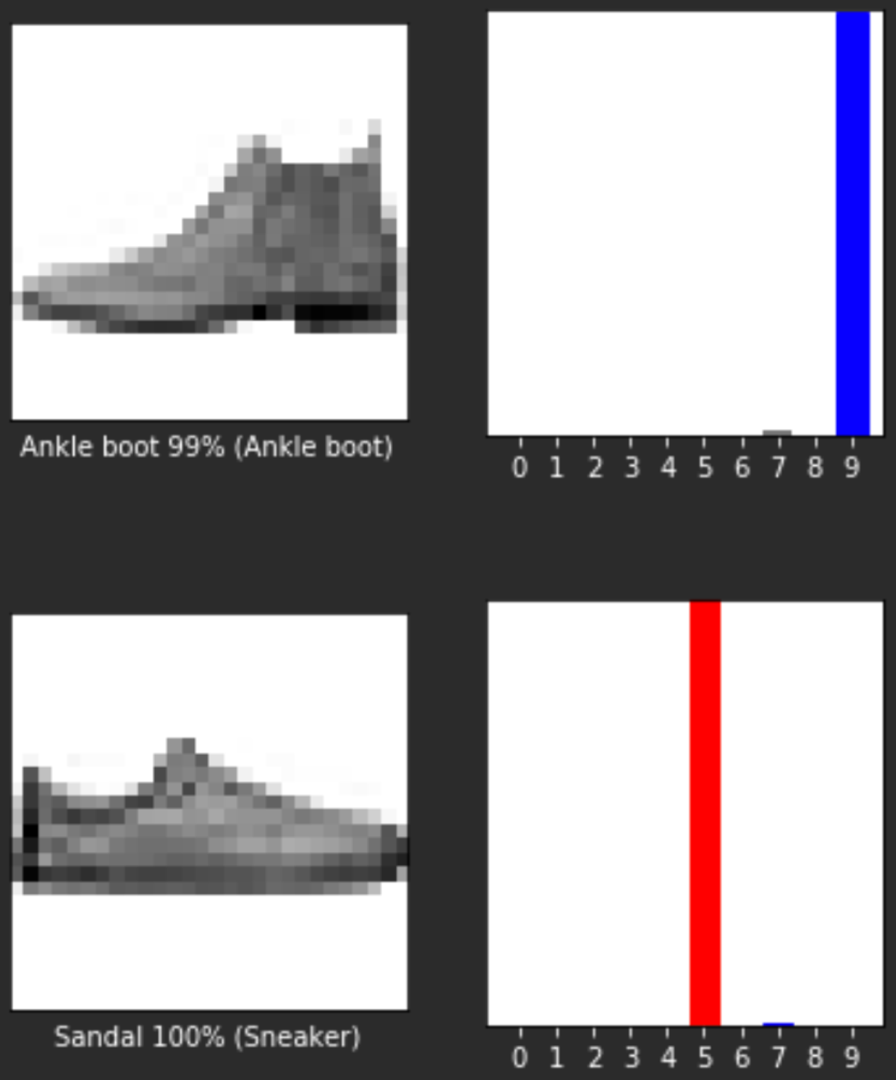
\includegraphics[width=0.45\textwidth]{classification.png}
        \end{center}
    \end{figure}

    \autoref{fig:classification} demonstrates the classification task.\ In this example, the top row indicates the classifier has successfully classified the image into the 9\textsuperscript{th} class (Ankle Boot).\ However, the bottom image has been misclassified into the 5\textsuperscript{th} class (Sandal) rather than the 7\textsuperscript{th} class (Sneaker).

    Classification was performed using two neural network architectures, one using only dense layers and another using convolutional layers.\ The first architecture, shown in~\autoref{fig:classifier-architecture-1}, flattens the 28x28 pixel image into a 784-pixel vector which is then densely connected to a 128-node layer;\ finally, the 128-node layer is densely connected to a 10-node output layer.

    \begin{figure}
        \caption{First Classifier Architecture}
        \label{fig:classifier-architecture-1}
        \begin{center}
            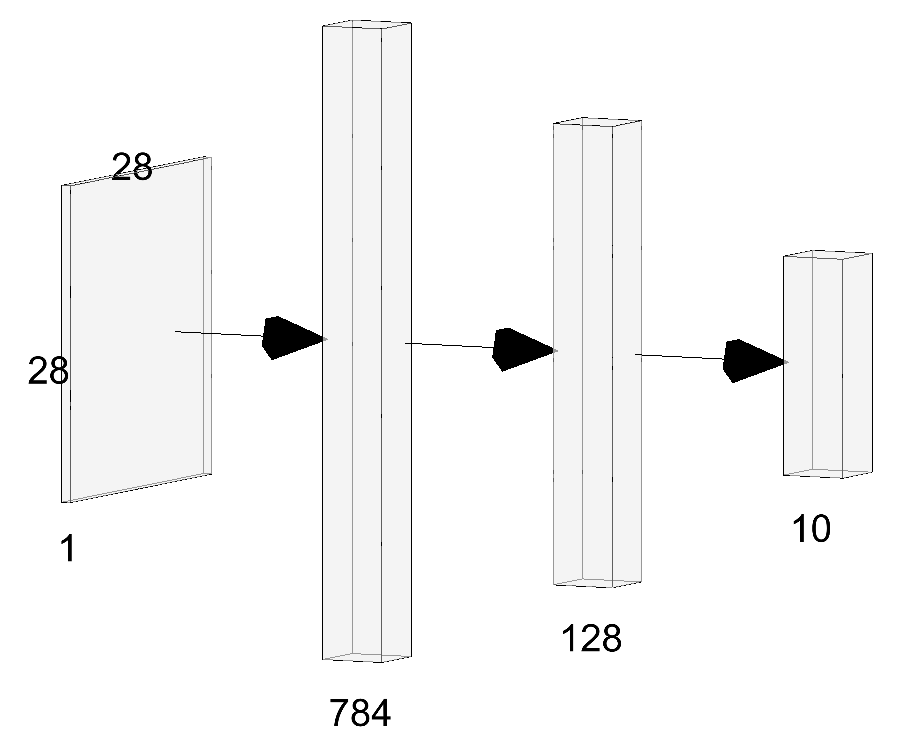
\includegraphics[width=0.45\textwidth]{First_Classifier_Architecture.png}
        \end{center}
    \end{figure}

    The second architecture, shown in~\autoref{fig:classifier-architecture-2}, scans the image with a convolutional neural network using a 5x5 window and 64 layers;\ the results of the first convolutional layer are then scanned by another convolutional layer with a 5x5 window and 128 layers.\ The final step is to flatten the layer and densely connect it to the 10-node output layer.

    \begin{figure}
        \caption{Second Classifier Architecture}
        \label{fig:classifier-architecture-2}
        \begin{center}
            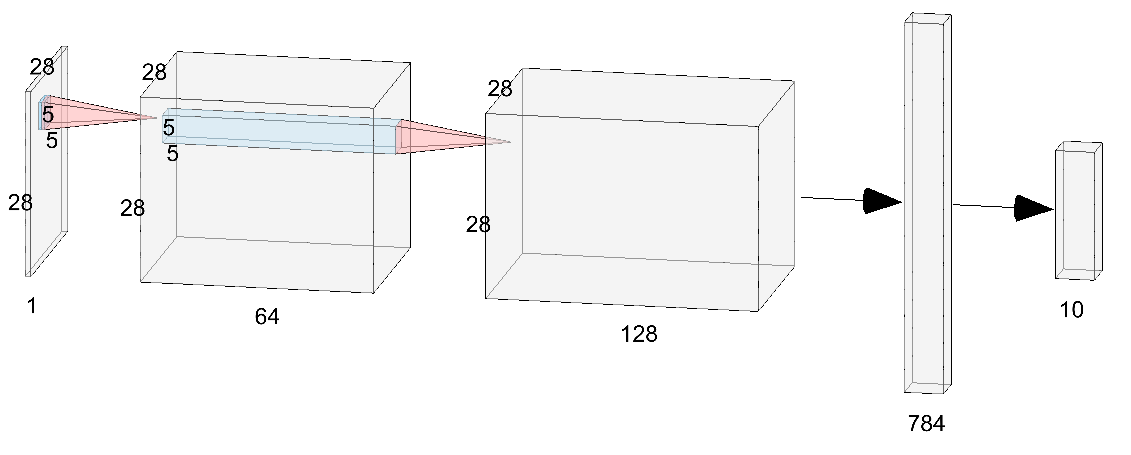
\includegraphics[width=0.45\textwidth]{Second_Classifier_Architecture.png}
        \end{center}
    \end{figure}

    The output layer of both architectures indicates the network's confidence that the image belongs to each of the classes, so a large value in the 0\textsuperscript{th} and 6\textsuperscript{th} nodes would indicate that the network is uncertain whether an image should be classified as a T-shirt/top or just a Shirt.\ The neural networks described were constructed using Keras and TensorFlow in Jupyter notebooks.

    The robustness of the classifier was tested by adding adversarial signals to the input images.\ The adversarial signal was calculated by determining the gradient of the loss function based on the input image used.\ This allows the adversarial signal to skew the image to the closest incorrect classification.\ Once the adversarial signal was determined, it was scaled by an \(\epsilon\) value (between 0 and 1) and added to the image;\ for adding this noise the image is considered to consistent entirely of pixels that have a brightness value greater than 0.\ Limiting the noise to non-zero values means the classification isn't being skewed due to noise added in the black background portions of the image.\ Robustness was determined by comparing the accuracy of our classifiers against ever-increasing \(\epsilon\) values.

    \subsection{Generation}\label{subsec:implementation-generation}

    A key goal from the onset of this project was to use GANs to generate images which are believable reproductions of those in fashion-mnist.\ During the planning stage, various projects which achieved the goal were identified as references.\ Two stood out above the rest: tensorflow-generative-model-collections~\cite{tensorflow-generative-model-collections} and pytorch-generative-model-collections~\cite{original-pytorch-generative-model-collections}.\ Both take the same approach of training ten different GANs on various datasets, including fashion-mnist.\ The PyTorch implementation proved easier to execute on the SJSU HPC due to its more modern dependency stack, therefore it was chosen as the foundation of the generative component of this project.

    The ten GANs explored for this project were:

    \begin{enumerate}
        \item Generative Adversarial Network (GAN; June 2014)~\cite{goodfellow2014generative}: The original GAN paper by Goodfellow, et al.\ introduced the world to the idea of training competing deep networks to improve generative models.
        \item Conditional GAN (CGAN; November 2014)~\cite{mirza2014conditional}: Followed an idea posed at the end of the original GAN paper to see how GANs might be used to fulfill conditional constraints such that the generated samples targeted a specific output class.
        \item Information Maximizing GAN (infoGAN; June 2016)~\cite{chen2016infogan}: Maximizes mutual information during training to learn features without supervision which can be tuned to alter characteristics of the generated models (i.e.\ shifting the angle of MNIST--like digits).
        \item Energy-based GAN (EBGAN; March 2017)~\cite{zhao2017energybased}: An energy-based approach to GANs that yielded promising results for high-resolution images.
        \item Auxiliary Classifier GAN (ACGAN; July 2017)~\cite{odena2017conditional}: Trains the generator to generate a classification for each sample it produces, eventually proving GANs can learn over numerous diverse classes with high-resolution images.\ It achieves especially impressive results on ImageNet.
        \item Least Squares GAN (LSGAN; April 2017)~\cite{mao2017squares}: Swaps out the sigmoid cross entropy loss function for the least squares loss function to avoid vanishing gradients, thereby forcing the generator to produce higher quality images.
        \item Wasserstein GAN (WGAN; January 2017)~\cite{arjovsky2017wasserstein}: A theoretically-dense paper which introduces the critic into the standard game between a generator and discriminator to achieve more durable training and avoid mode collapse.
        \item Boundary Equilibrium GAN (BEGAN; May 2017)~\cite{berthelot2017began}: Stabilizes training via an equilibrium, but more interestingly, explores the inverse relationship between diversity of generated images (modality) and image quality.
        \item Wasserstein GAN - Gradient Penalty (WGAN\_GP; December 2017)~\cite{gulrajani2017improved}: Enables training deeper, more complicated networks than previously possible by removing critic weight clipping from WGAN in favor of gradient penalties.
        \item Deep Regret Analytic GAN (DRAGAN; December 2017)~\cite{kodali2017convergence}: Calls into question the assumption that modality and quality are inversely correlated.
    \end{enumerate}

    Each was trained independently on the fashion-mnist dataset for fifty epochs.\ The loss metric was tracked for each training session.\ To communicate the results of the training process more coherently, a snapshot of images produced by the generator is saved at the end of each epoch as demonstrated in \autoref{fig:generation-gan}.\ Upon completion, each set of fifty images was compiled into a GIF to aid comprehension.

    \subsection{Colorization}\label{subsec:implementation-colorization}

    The images in the fashion-mnist dataset are all grayscale images.\ We decided to build a machine learning model that would fill colors into these grayscale images intelligently.\ There exist several techniques available to fill static colors into them;\ however, our goal is to have the model learn to color the images intelligently.\ We decided to use GANs~\cite{colorization_GAN} to perform this task.

    To build a model capable of intelligently colorizing grayscale images, we had to first build a dataset for training our GAN model.\ We combined the training and testing sets of the fashion-mnist dataset.\ Next, we filled colors into these 70,000 grayscale images as seen in \autoref{fig:colorization}.\ Initially, the shape of each image was (28,28,1).\ After colorizing the images, their shape changed to (28,28,3).\ The additional rows hold the red, green, and blue pixel values.\ Each label of the fashion-mnist dataset was assigned different colors.\ For instance, ankle boots were colored brown and dresses were colored red.\ Now, all 70,000 data points in fashion-mnist have been transformed into (28,28,3) matrices to hold colorized representations~\cite{initexploration}.

    \begin{figure}
        \caption{Training Samples for Colorization}
        \label{fig:colorization}
        \centering
        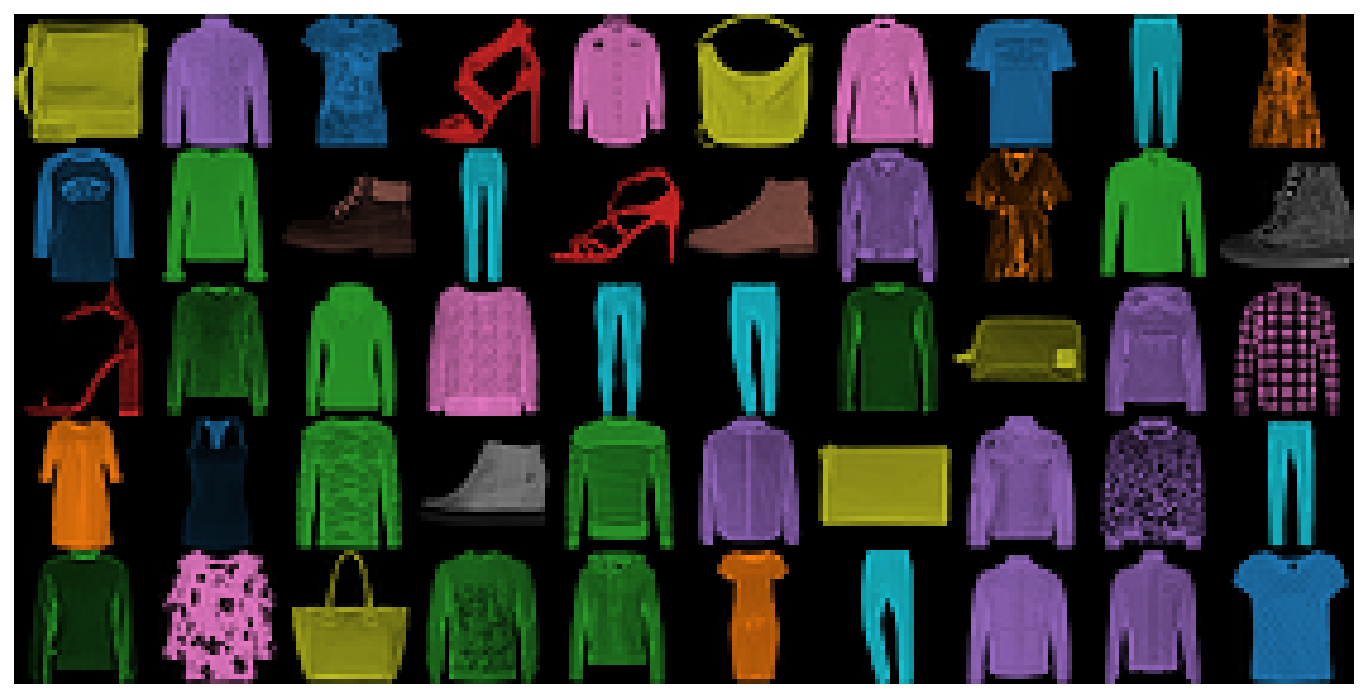
\includegraphics[width=0.45\textwidth]{Colorization_training_samples.png}
    \end{figure}

    Once the training samples were created, experiments with GANs commenced~\cite{coloringimages}.\ The original grayscale images were input to the generator.\ The generator then tried to fill colors into these grayscale images using some randomly set weights.\ These generated images were then passed on to the discriminator.\ Along with these images, the discriminator also received the explicitly colored images from the training sample.\ The discriminator tried to identify which image was created from the generator and which was drawn from the training sample.\ Based on the decision made on the classification task by the discriminator, the discriminator loss as well as the generator loss were computed.

    The discriminator in the network learnt from the discriminator loss by backpropagating through the discriminator node and updating the weights associated with the discriminator.\ Similarly, the generator updated its weights using the results obtained from backpropagating through the generator node and using the generator loss.\ This process of updating the weights and learning was carried out iteratively.\ After running this iterative process for certain epochs, we had the final weights for the network that were capable of colorizing the items in the fashion mnist dataset intelligently.

    We used DCGANs~\cite{dcgans} to define the neural network model.\ The DCGANs architecture displayed in \autoref{fig:dcgan-architecture} gives a low level overview of the model used for colorizing the grayscale images of the fashion mnist dataset.\ It introduces the generators and discriminators along with the training process step by step.

    \begin{figure}
        \caption{DCGAN Architecture}
        \label{fig:dcgan-architecture}
        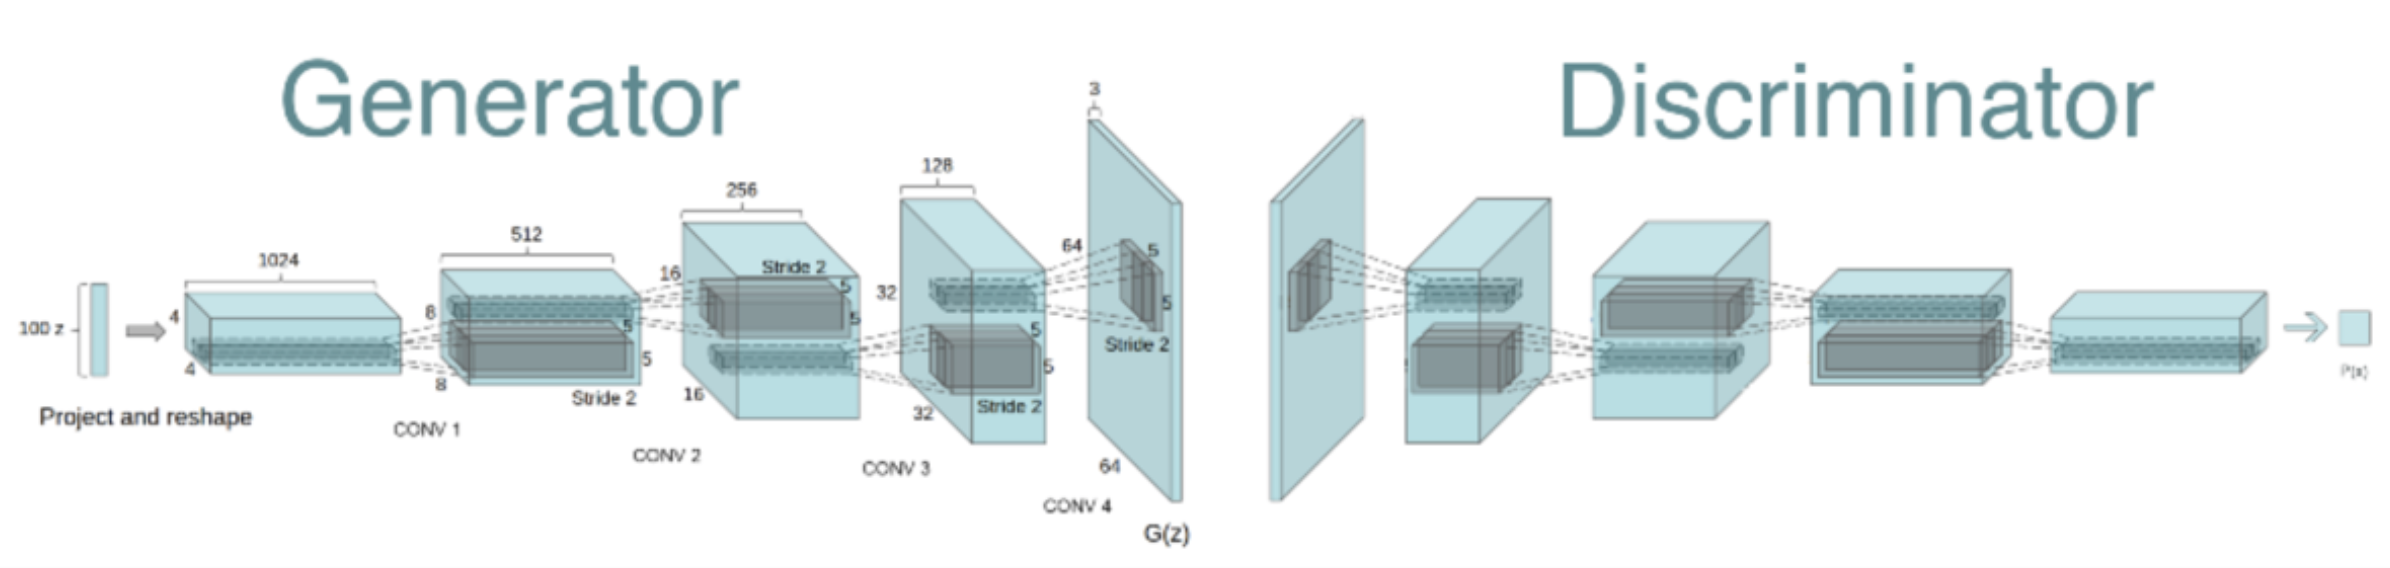
\includegraphics[width=0.45\textwidth]{architecture.png}
        \centering
    \end{figure}

    DCGANs use a random noise vector as input, and the input is then scaled up into two-dimensional data similar to CNN's but in the opposite structure.\ For non-linear layers, we recommend using LeakyReLU for all layers for the discriminator.\ For the generator, we found that the BatchNormalize layer was the optimal choice, primarily because using BatchNormalize allows the CNN version of the generator to learn better, but it is impossible to use BatchNormalize for all layers.\ The output layer of the generator and input layer of the discriminator do not require a BatchNormalize layer.\

    Parameter setting for our project:

    \begin{itemize}
        \item batch size: 64
        \item Used Adam optimizer instead of Root Mean Square Propagation optimizer
        \item iteration times: 20000
        \item learning rate: 0.0001
        \item BatchNormalization: momentum=0.9
    \end{itemize}

    \section{Results}\label{sec:results}

    \subsection{Classification}\label{subsec:results-classification}

    Both classifiers had a training accuracy of 91\%, and a test accuracy around 90\%, 88\% for the dense network and 90\% for the convolutional network.\ This indicates we had some slight overfitting, but overall both classifiers performed well.\ The classifiers also seem to be fairly robust, since with an epsilon value of 0.05 we still saw a classification accuracy of 75\%.~\autoref{fig:adversarial-noise-accuracy} shows the accuracy of our classifiers as epsilon is increased.
    \begin{figure}
        \begin{center}
            \caption{Accuracy with Adversarial Noise}
            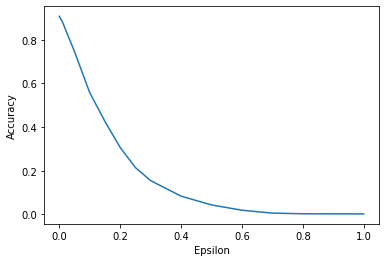
\includegraphics[width=0.45\textwidth]{Adversarial Accuracy.png}
            \label{fig:adversarial-noise-accuracy}
        \end{center}
    \end{figure}
    The adversarial noise can be visually noticed with an epsilon of 0.1, so maintaining a 75\% accuracy rate when the visual noise is largely unnoticeable to human observers is fairly robust.\ Based on the work of Goodfellow, Schlens, and Szegedy, the epsilon values at which adversarial noise effects a dataset is rather small~\cite{adversarialexamples}.\ Their classifier for the traditional MNIST data set produces an error rate of 89.4\% with an epsilon of 0.25, and an error rate of 87\% with an epsilon of 0.1.\ The difference in our accuracy compared to theirs is probably due to filtering the adversarial noise to only be on the image rather than in the black background as well.\ The main issues for the classifiers seem to be the similarity between some of the classes.\ The classifier has lower confidence in distinguishing between t-shirt and shirt, and between some sandals and ankle boots.\ It could be interesting to see how the classifier changes if some of these groups are joined together.

    \subsection{Generation}\label{subsec:results-generation}

    The results of the original implementation were fully replicated.\ The presentation we delivered contains all of our results;\ a select few have been selected for this report.

    After reading the ten papers in which these architectures are described, we could interpret the results more astutely.\ For instance, a common problem articulated by many of the papers is the challenge of training stability.\ They describe the fragility of the balance that exists between the discriminator and generator.\ Many of the papers specifically focus on ways to synchronize their learning, so the discriminator doesn't outpace the generator too early.\ The plots all tell that story;\ the discriminator's loss always improves faster than the generator.\ Notably, however, the research into training stability can be visually seen.\ In \autoref{fig:loss-plot-wgan}, the more modern WGAN keeps the discriminator and generator in balance rather than allowing them to diverge as with the original GAN shown in \autoref{fig:loss-plot-gan} or CGAN shown in \autoref{fig:loss-plot-cgan}.

    Another interesting observation manifest in the results is that GANs can learn to model specific classes.\ The original GAN does not constrain its generator to a particular output class, therefore it can be observed to shift its output based on the likelihood of fooling the discriminator in \autoref{fig:generation-gan};\ look specifically at the image directly to the right of the top-left corner (i.e.\ row 0, column 1) to see the generator switch from producing a Shirt to a Bag.\ In contrast, CGAN permits learning only on specified classes.\ Each column of \autoref{fig:generation-cgan} holds predictions in a distinct output class.

    Between \autoref{fig:generation-gan}, \autoref{fig:generation-cgan}, and \autoref{fig:generation-wgan}, it seems the most recent (WGAN) actually produces the lowest quality predictions.\ Why?\ We suspect that its attempts to avoid mode collapse (the tendency for a GAN's predictions pool increasingly around a few high-confidence output classes) come at the cost of granularity.\ Of course, the DRAGAN authors would disagree.\ Ultimately, we need to perform additional research to understand this property of GANs better.

    \begin{figure}
        \caption{GAN Generations}
        \label{fig:generation-gan}
        \centering
        \subfloat[\centering Epoch 1]{{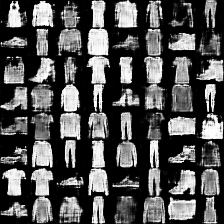
\includegraphics[width=0.15\textwidth]{GAN_epoch001.png} }}
        \subfloat[\centering Epoch 25]{{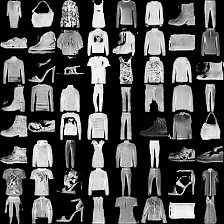
\includegraphics[width=0.15\textwidth]{GAN_epoch025.png} }}
        \subfloat[\centering Epoch 50]{{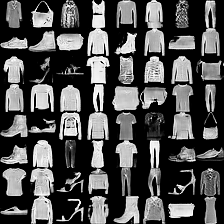
\includegraphics[width=0.15\textwidth]{GAN_epoch050.png} }}
    \end{figure}

    \begin{figure}
        \caption{CGAN Generations}
        \label{fig:generation-cgan}
        \centering
        \subfloat[\centering Epoch 1]{{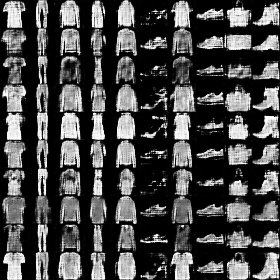
\includegraphics[width=0.15\textwidth]{CGAN_epoch001.png} }}
        \subfloat[\centering Epoch 25]{{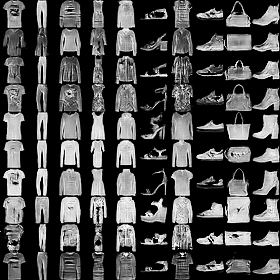
\includegraphics[width=0.15\textwidth]{CGAN_epoch025.png} }}
        \subfloat[\centering Epoch 50]{{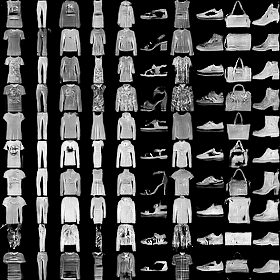
\includegraphics[width=0.15\textwidth]{CGAN_epoch050.png} }}
    \end{figure}

    \begin{figure}
        \caption{WGAN Generations}
        \label{fig:generation-wgan}
        \centering
        \subfloat[\centering Epoch 1]{{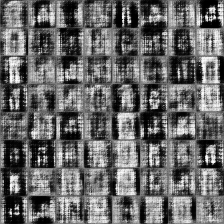
\includegraphics[width=0.15\textwidth]{WGAN_epoch001.png} }}
        \subfloat[\centering Epoch 25]{{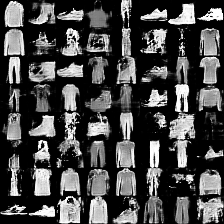
\includegraphics[width=0.15\textwidth]{WGAN_epoch025.png} }}
        \subfloat[\centering Epoch 50]{{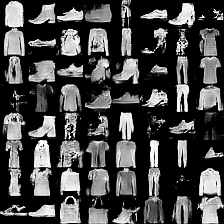
\includegraphics[width=0.15\textwidth]{WGAN_epoch050.png} }}
    \end{figure}

    \begin{figure}
        \caption{GAN Loss Plot}
        \label{fig:loss-plot-gan}
        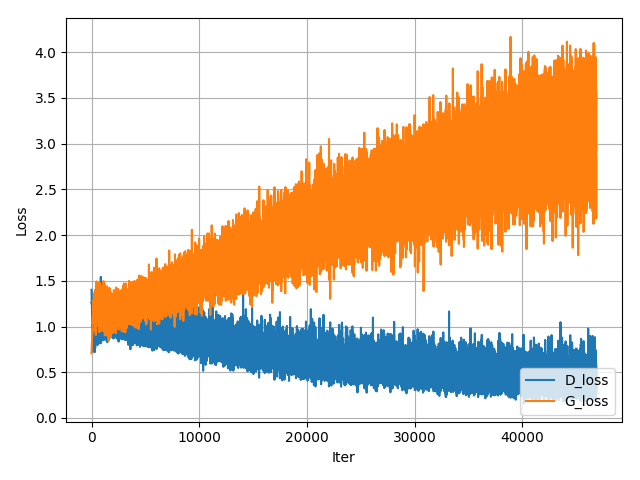
\includegraphics[width=0.45\textwidth]{GAN_loss.png}
        \centering
    \end{figure}

    \begin{figure}
        \caption{CGAN Loss Plot}
        \label{fig:loss-plot-cgan}
        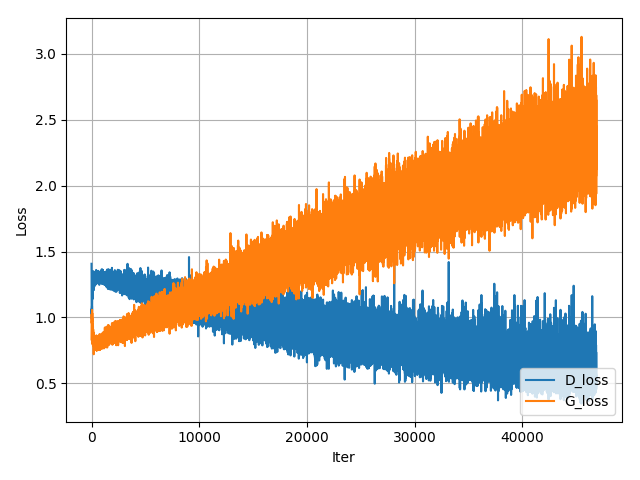
\includegraphics[width=0.45\textwidth]{CGAN_loss.png}
        \centering
    \end{figure}

    \begin{figure}
        \caption{WGAN Loss Plot}
        \label{fig:loss-plot-wgan}
        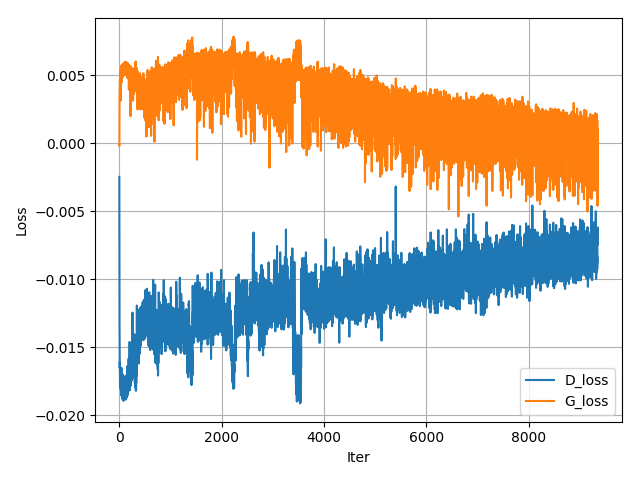
\includegraphics[width=0.45\textwidth]{WGAN_loss.png}
        \centering
    \end{figure}

    \subsection{Colorization}\label{subsec:results-colorization}

    TODO: Cite~\cite{e-in-style}.
    TODO: Cite~\cite{pytorch-generative-model-collections}.

    With the structure of the generative model and the discriminant model of the CNN structure provided in \autoref{fig:dcgan-architecture} and training samples similar to \autoref{fig:colorization}, the results achieved by our model can be seen in \autoref{fig:colorized_result}.

    \begin{figure}
        \caption{Colorized Clothing Images}
        \label{fig:colorized_result}
        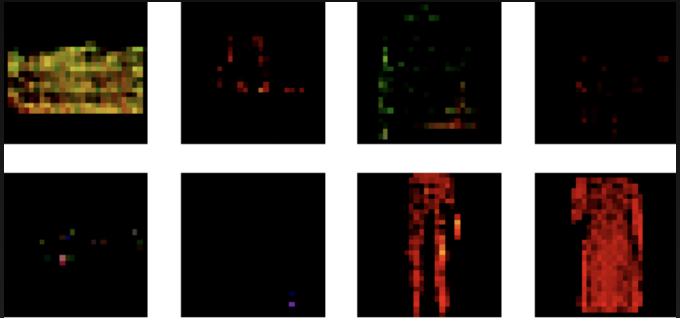
\includegraphics[width=0.45\textwidth]{learned_result.png}
        \centering
    \end{figure}

    It can be clearly seen that the generated images are not as good as the black and white examples, mainly due to the difficulty in setting up the training set.\ We tried replacing too many background images and ended up using this new dataset.\ The generator must generate clothing images and have a valid background (retrieved from real images).\ With more training, additional training samples or some special techniques, one might be able to improve the generated images.\ However, since this is one way to use GAN to adapt to RGB images, we are delighted with the results.

    For our project, we have used DCGAN to generate colorful clothing images.\ One can try to change the dataset to generate images that suits their personal need, or try to modify the neural network parameters to observe different generation effects.\ The size of non-trainable parameters in Adam optimizer was larger than RMSprop.\ This result excludes all parameters of the discriminator.\

    \section{Conclusion}\label{sec:conclusion}

    As evidenced by the diverse branches this project explored, neural networks are largely deserving of the hype they receive.\ We successfully leveraged them to perform multi-class classification and generative modeling over fashion-mnist.\ Furthermore, the breadth of GAN architectures provided broad exposure to modern research trends and problems GANs still face.\ No breakthrough theoretical discoveries were made.\ Nonetheless, our experiments and results lent us critical insight into the forces governing these techniques.

    \bibliographystyle{ieeetr}
    \bibliography{report}
\end{document}
